% Options for packages loaded elsewhere
\PassOptionsToPackage{unicode}{hyperref}
\PassOptionsToPackage{hyphens}{url}
%
\documentclass[
]{article}
\usepackage{lmodern}
\usepackage{amssymb,amsmath}
\usepackage{ifxetex,ifluatex}
\ifnum 0\ifxetex 1\fi\ifluatex 1\fi=0 % if pdftex
  \usepackage[T1]{fontenc}
  \usepackage[utf8]{inputenc}
  \usepackage{textcomp} % provide euro and other symbols
\else % if luatex or xetex
  \usepackage{unicode-math}
  \defaultfontfeatures{Scale=MatchLowercase}
  \defaultfontfeatures[\rmfamily]{Ligatures=TeX,Scale=1}
\fi
% Use upquote if available, for straight quotes in verbatim environments
\IfFileExists{upquote.sty}{\usepackage{upquote}}{}
\IfFileExists{microtype.sty}{% use microtype if available
  \usepackage[]{microtype}
  \UseMicrotypeSet[protrusion]{basicmath} % disable protrusion for tt fonts
}{}
\makeatletter
\@ifundefined{KOMAClassName}{% if non-KOMA class
  \IfFileExists{parskip.sty}{%
    \usepackage{parskip}
  }{% else
    \setlength{\parindent}{0pt}
    \setlength{\parskip}{6pt plus 2pt minus 1pt}}
}{% if KOMA class
  \KOMAoptions{parskip=half}}
\makeatother
\usepackage{xcolor}
\IfFileExists{xurl.sty}{\usepackage{xurl}}{} % add URL line breaks if available
\IfFileExists{bookmark.sty}{\usepackage{bookmark}}{\usepackage{hyperref}}
\hypersetup{
  pdftitle={Choosing an answer strategy},
  hidelinks,
  pdfcreator={LaTeX via pandoc}}
\urlstyle{same} % disable monospaced font for URLs
\usepackage[margin=1in]{geometry}
\usepackage{graphicx,grffile}
\makeatletter
\def\maxwidth{\ifdim\Gin@nat@width>\linewidth\linewidth\else\Gin@nat@width\fi}
\def\maxheight{\ifdim\Gin@nat@height>\textheight\textheight\else\Gin@nat@height\fi}
\makeatother
% Scale images if necessary, so that they will not overflow the page
% margins by default, and it is still possible to overwrite the defaults
% using explicit options in \includegraphics[width, height, ...]{}
\setkeys{Gin}{width=\maxwidth,height=\maxheight,keepaspectratio}
% Set default figure placement to htbp
\makeatletter
\def\fps@figure{htbp}
\makeatother
\setlength{\emergencystretch}{3em} % prevent overfull lines
\providecommand{\tightlist}{%
  \setlength{\itemsep}{0pt}\setlength{\parskip}{0pt}}
\setcounter{secnumdepth}{-\maxdimen} % remove section numbering
\usepackage{booktabs}
\usepackage{longtable}
\usepackage{array}
\usepackage{multirow}
\usepackage{wrapfig}
\usepackage{float}
\usepackage{colortbl}
\usepackage{pdflscape}
\usepackage{tabu}
\usepackage{threeparttable}
\usepackage{threeparttablex}
\usepackage[normalem]{ulem}
\usepackage{makecell}
\usepackage{xcolor}

\title{Choosing an answer strategy}
\author{}
\date{\vspace{-2.5em}}

\begin{document}
\maketitle

{
\setcounter{tocdepth}{4}
\tableofcontents
}
\hypertarget{choosing-an-answer-strategy}{%
\section{Choosing an answer
strategy}\label{choosing-an-answer-strategy}}

Your answer strategy is your plan for what you will do with the
information gathered from the world in order to generate an answer to
the inquiry. Qualitative and quantitative methods courses overflow with
advice about which answer strategies to choose. Under what conditions
should you use Ordinary Least Squares, when should you use logit? When
is a machine learning algorithm the appropriate choice and when would a
comparative case study be more informative? When is \emph{no} answer
strategy worth pursuing because of the fundamental limitations of the
data strategy?

Our perspective on answer strategies is that they should be informed by
the other three elements of research design: the model, the inquiry, and
the data strategy. Sometimes answer strategy advice is offered on the on
the basis of the realized data \(d\) only, without any particular
attention paid to important features of the question to be answered or
the manner in which the data were collected and generated. For example,
a bit of received methodological wisdom holds that whenever a dependent
variable is binary, a binary choice statistical model like logit or
probit must be used. This advice is based only the knowledge that \(d\)
contains a binary outcome; whether it is appropriate depends on features
of \(I\) and features of \(D\). For example, if \(I\) is the average
treatment effect and \(D\) includes randomization of the treatment,
answer strategies beyond binary choice models may serve just as well or
better. If a student asks, ``which estimator should I use?'' the
response is always, ``it depends.'' What does it depend on? The model,
the inquiry, and the data strategy.

Choosing ``design-aware'' answer strategies sounds straightforward
enough, but the precise way in which this approach is applied in any
real empricial setting will of course differ from case to case. Our
highest-level advice is that we want to pick an answer strategy \(A\)
such that the answer it provides \(A(d) = a^d\) is close to the answer
under our model of the world, \(I(m) = a^m\). The implication is that we
should strive for parallelism across \(A\) and \(I\). This idea
sometimes described as the ``plug-in principle.'' When the function
\(A\) is very close to the function \(I\), then we can ``plug in'' \(d\)
for \(m\). Following the plug-in principle leads to very straightforward
estimation procedures. If the inquiry is a population mean, we can use
the sample mean estimator to estimate it, so long as the data strategy
produces data \(d\) that are sufficiently representative of \(m\). To
the extent possible, we want to choose data strategies that enable
plug-in estimator answer strategies.

At some level, all answer strategies rely on unverifiable but hopefully
plausible assumptions. For descriptive inference, we have to assume that
the sample represents the population well. For causal inference, we have
to assume that treated and untreated units are similar in all other
respects beyond treatment status. For all kinds of inference, we have to
assume that our measurements are close to the latent construsts we wish
to measure. Answer strategies are \emph{model-based} when the most
consequential of these assumptions are part of \(M\). Answer strategies
are \emph{design-based} to the extent that we can pull the assumptions
out of \(M\) and assure them by design, i.e., by choosing \(D\) in such
a way that we can be confident that the assumption is true.
Observational causal inference often relies on an assumption of
``selection on observables,'' or the claim that within groups of units
that have the same observed characteristics, treatments are as-if
randomly assigned. Observational causal inference is model-based in the
sense that the selection on observables assumption is grounded in
researchers' theoretical model of the world, which of course might be
wrong. Experimental causal inference is design-base in the sense that we
can be sure that treatments were indeed randomly assigned because random
assignment was part of the data strategy. In both observational and
experimental settings we need to make the same assumption, but in one
case, we rely on a theoretical model and in the other, we rely on a data
strategy. Where possible, we prefer assuring assumptions by design to
asserting them on the basis of a theoretical model.

Answer strategies come in a number of varieties. The most familiar of
these are point-estimators that produce estimates of parameters.
Ordinary least squares, difference-in-means, logit, random forests, and
a very long list of others are in the point-estimator answer strategy
class. A second class is comprised of tests. Tests return a binary
decision (True or False). Null hypothesis significance tests are a
common form of test in quantitative research. Qualitative researchers
also employ tests; these go by names like ``hoop test'' and
``straw-in-the-wind'' test. Bayesian answer strategies return full
posterior distributions. In contrast to point-estimators some answer
strategies are interval-estimators. Which class of estimator to choose
-- and which particular estimator within the class you select -- will
depend on features of your model, inquiry, and data strategy. The
sections to follow walk through some of the most important ways these
design features influence the answer strategy, though they will by no
means offer a full accounting. The range of estimation of approaches is
vast and this book is not the place to tally each of their strengths and
weaknesses. Instead, our goal is to provide a framework for thinking
about how you would go about choosing one answer strategy over another.

\hypertarget{following-the-model}{%
\subsection{Following the model}\label{following-the-model}}

As we described in chapter 6, we can (non-parametrically) express our
model of the world as a directed acyclic graph, or DAG. DAGs express
\emph{some} but not all parts of our model, precisely because they are
nonparametric. They don't encode how variables cause each other, just
whether they do. Even so, writing down a theoretical model in as
parsimonious a form as a nonparametric structual causal model can guide
answer strategies in an enormously powerful way. Given a DAG, we can
learn whether \emph{any} answer strategy would be sufficient for
estimating a causal effect. Further, we can learn which variables our
answer strategy must condition on, and which must be left alone.

When we want to estimate a particular causal relationship, such as the
average causal effect of D on Y, we can read off the DAG whether that
relationship is \emph{identified} or not. The most common (and useful)
criterion for identification is the ``backdoor criterion.'' If there
exists an unblocked ``backdoor path'' from D to Y, then the relationship
is not identified.\footnote{Footnote here about other criteria.} A
backdoor path is a causal path that begins with an arrow in to D and
ends with an arrow in to Y. Backdoor paths can be blocked in two ways:
conditioning the analysis on a variable along the path or \emph{not}
conditioning on a ``collider'' along the path.

Pearl (p.~61) defines the backdoor criterion:

Given an ordered pair of variables D, Y in a DAG G, a set of variables
X, satifies the backdoor criterion relative to D, Y if no node in X is a
descendant of D, and X blocks every path between D and Y that contains
an arrow into D. (pg. 61 Pearl primer)

With this definition in hand, we can inspect DAGs to find ``adjustment
sets.'' An adjustment set is a set of variables that may be conditioned
upon in the answer strategy. ``Conditioned upon'' is a sufficiently
vague phrase to include conditioning procedures such as controlling for
a variable in a regression setting or stratifying the analysis according
to those variables.

In general, if \(X\) is an adjustment set that satisfies the backdoor
criterion, then we can estimate the conditional probability
distributions of \(Y\) for each level of \(D\) using this expression.

\[\Pr(Y = y \mid do(D=d)) = \sum_x \Pr(Y = y \mid D = d, X = x) \Pr(X = x)\]

We can write the same expression using potential outcomes notation:

\[\Pr(Y_i(D_i = 1) = y) = \sum_x \Pr(Y_i(D_i = 1) = y \mid X_i = x) \Pr(X_i = x)\]

Figure @ref(fig:threedags) shows three DAGs with these three variables
D, X, and Y, as well as an additional unmeasured variable \(U\) (we will
consider \(U\) in later sections). In all three cases, our inquiry is
the average treatment effect of D on Y, and in all three cases, X, D,
and Y are correlated. In the first case, \(X\) confounds the causal
relationship between D and Y, which is to say if we simply compared
units with different levels of D, our estimates of the causal effect
would be prone to bias. However, if we conduct the analysis separately
\emph{within} levels of X (that is to say, we condition on X), then
combine the separate analyses, our overall estimate will be unbiased.
This first DAG is the setting that analysts have in mind when
controlling for observables in order to estimate causal effects.

A dangerous possibility, however, is represented by the second DAG. In
this causal graph, X doesn't confound the relationship between D and Y
-- instead, it is a downstream consequence of both variables. If an
analyst mistakenly conditions on X, a noncausal confounding path opens
up between D and Y, biasing estimates of average effect on D on Y. The
contrast between the first and second graphs is an illustration of the
general principle that our theoretical models guide analytic choices. In
the first case, our estimates are unbiased if and only if we \emph{do}
control for \(X\), in the second case if and only if we \emph{do not}
control for X.

The third case describes a setting in which D has both a direct effect
on Y and an indirect effect that travels through X -- in this case, X is
a mediator. If we condition on X, our estimate of the effect D on Y is
biased (X is a descendant of D). Like in the collider case, the effect
is identified if we \emph{do not} control for X, but is not identified
if we \emph{do} condition. Some intuition for the problems associated
with controlling for mediators: controlling for X ``controls away'' some
portion of the effect.

This example illustrates in a small way how your model of the world
guides your answer strategy. In all three cases, we could in principle
have the same dataset of D, X, and Y. If we followed some common
regression advice, we would control for X in all three cases because it
is correlated with both D and Y -- this approach works only if X is a
confounder. If X is a collider or a mediator, then this control strategy
would induce bias. Without further changes to the design, no empirical
tests can distinguish between these three DAGs, so in a very real way,
theoretical assumptions in the Model must be relied upon to correctly
choose a control strategy.

\begin{figure}
\centering
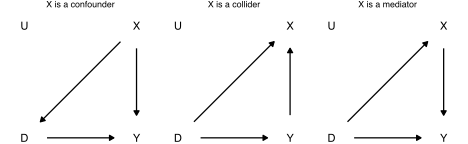
\includegraphics{05_Choosing_an_Answer_Strategy_files/figure-latex/threedags-1.pdf}
\caption{Three roles for a variable X.}
\end{figure}

We consider three possible paths to estimating the effect of the
treatment \(D\) on \(Y\). First, we consider conditioning on \(X\)
without making additional assumptions about the DAG; second, we consider
invoking an ignorability assumption, often known as
selection-on-observables; third, we consider randomizing the treatment
and measuring \(X\) before treatment. Finally, we consider the role of
estimation in narrowing down the set of possible DAGs that describe the
world.

\hypertarget{identification}{%
\subsubsection{Identification}\label{identification}}

We can only learn the answer to the inquiry when we can \emph{identify}
the causal effect, meaning if we had infinite data we could estimate
without bias the causal effect. Identification can be obtained if the
backdoor criterion is met, if the frontdoor criterion is met, or if
there are no other causal relationships into both \(D\) and \(Y\). These
conditions will be violated in several circumstances, including when an
observed confounder \(X\) confounds the relationship between \(D\) and
\(Y\) and is left unadjusted or when there is an unobserved confounder
\(U\).

To reason about causal identification, we turn back to DAGs. We start
with a simple DAG with four variables: a treatment \(D\), an outcome
\(Y\), a observed variable \(X\) (which may or may not confound the
relationship between \(D\) and \(Y\)), and an unobserved variable \(U\).
There are six edges between these variables, each with three possible
relations: each variable may cause (e.g., \(D \rightarrow Y\)), be
caused by (e.g., \(D \leftarrow Y\)), or not be causally related to
every other variable. With three possible relationships and six edges,
there are \(3^6 = 729\) conceptually possible DAGs. We rule out DAGs in
which other variables cause \(U\), because we defined \(U\) as an
unobserved confounder. This leaves 216 possible combinations. We do not
know which one! Our goal as researchers is to narrow down the possible
DAGs.

To do so, we collect data on the three observable variables, as in Table
@ref(fig:identificationsimdf). We are faced with the choice of answer
strategy. In the presence of possible confounding from \(X\) and/or
\(U\), we have several options for our research design: we can estimate
the causal effect of \(D\) on \(Y\) by controlling for the observed
confounder \(X\) (or not), by invoking additional conditional
independence assumptions, and by randomizing the treatment. In each
case, our aim is to rule out DAGs in which the causal effect is not
identified.

\begin{table}

\caption{\label{tab:identificationsimdf}Simulated data from a DAG with varaibles $X$, $D$, $Y$, and $U$.}
\centering
\begin{tabular}[t]{l|r|r|r}
\hline
ID & X & D & Y\\
\hline
001 & 0.531 & 1 & 2.240\\
\hline
002 & 0.181 & 0 & -1.278\\
\hline
003 & 0.777 & 0 & 1.154\\
\hline
004 & -0.576 & 0 & -0.998\\
\hline
005 & 0.661 & 0 & 0.682\\
\hline
006 & 1.270 & 0 & 0.434\\
\hline
\end{tabular}
\end{table}

\hypertarget{consequences-of-conditioning}{%
\paragraph{Consequences of
conditioning}\label{consequences-of-conditioning}}

The first strategy is that we can control for the observed variable
\(X\) or not. Whether controlling for \(X\) enables, prevents, or does
not affect the causal identification of the effect of \(D\) on \(Y\)
depends on our beliefs about which DAG is the true DAG.

We illustrate possible beliefs about these edges by visualizing all of
the 216 DAGs in which \(U\) is an unobserved confounder (see Figure
@ref(fig:dagsadjustment)). The large groups of three squares of nine
group DAGs based on how \(U\) affects other variables in the model: the
top left grouping of 27 DAGs represents those in which \(U\) affects all
of \(D\), \(X\) and \(Y\). Within that grouping, there are three squares
of nine squares. Each group of nine squares represents a set of DAGs
with a single relationship between \(D\) and \(Y\). The top left group
of nine are those DAGs in which \(D\rightarrow Y\).

We can rule out several of these 216 through acyclicity: the gray
squares are graphs that are cyclical. (We operate under the view that
cycling is not possible in the world, which would imply that these
variables simultaneously cause each other.)

We color the rest of the squares in terms of whether controlling for
\(X\) will identify the causal effect of \(D\) on \(Y\).

In some cases, the effect of \(D\) on \(Y\) will be identified
regardless of whether we control for \(X\) (white squares). For example,
in the left DAG, \(X\) affects \(D\) and \(U\) affects \(Y\) but neither
affect both. The causal effect is identified because there is no path
between \(D\) and \(Y\) except for the direct effect \(D\rightarrow Y\).
In other words, neither \(X\) nor \(U\) confound the relationship, and
the potential outcomes of \(Y\) are independent of \(D\).

In other cases, the effect of \(D\) on \(Y\) is identified if and only
if we control for \(X\) (blue squares). These are situations in which
\(X\) confounds the relationship and there is no additional confounding
from unmeasured confounders. These are cases in which the potential
outcomes of \(Y\) are independent of \(D\) \emph{conditional} on \(X\).

However, conditioning on \(X\) is risky, because if we are not in one of
the blue DAGs we might be in the purple DAGs in which the effect of
\(D\) on \(Y\) is identified only if we do \emph{not} condition on \(X\)
(purple squares). These are DAGs in which \(X\) is a collider, opening a
backdoor path between \(D\) and \(Y\) aside from the direct effect when
\(X\) is conditioned on. If we knew we were in one of these DAGs, we
would not control for \(X\).

There are also many situations --- a majority in fact, the pink squares
--- in which the relationship between \(D\) and \(Y\) is \emph{never}
identified, regardless of whether you control for \(X\). Most of these
result from confounding from unobservable confounders \(U\). The upper
left quadrant contains the cases where \(U\) affects all of the other
variables, and the middle left those where \(U\) affects \(D\) and
\(Y\). In both cases, identification would require at a minimum the
ability to control for these unmeasured confounders. The other
situations in which causal identification fails are those in which the
causal order between \(D\) and \(Y\) is reversed, i.e.~\(Y\) causes
\(D\). Without additional assumptions or control of the order in which
variables are collected from the data strategy, we cannot rule out this
possibility, the first and fourth columns of subgraphs labeled
\(D\leftarrow Y\).

Without additional assumptions or manipulation in our data strategy, we
cannot know where we are among the 200 acyclic DAGs represented in the
plot. As a result, we are in danger either of having the effect of \(D\)
on \(Y\) unidentified regardless of what we do, or of making the wrong
choice to control or not to control.

\begin{figure}
\centering
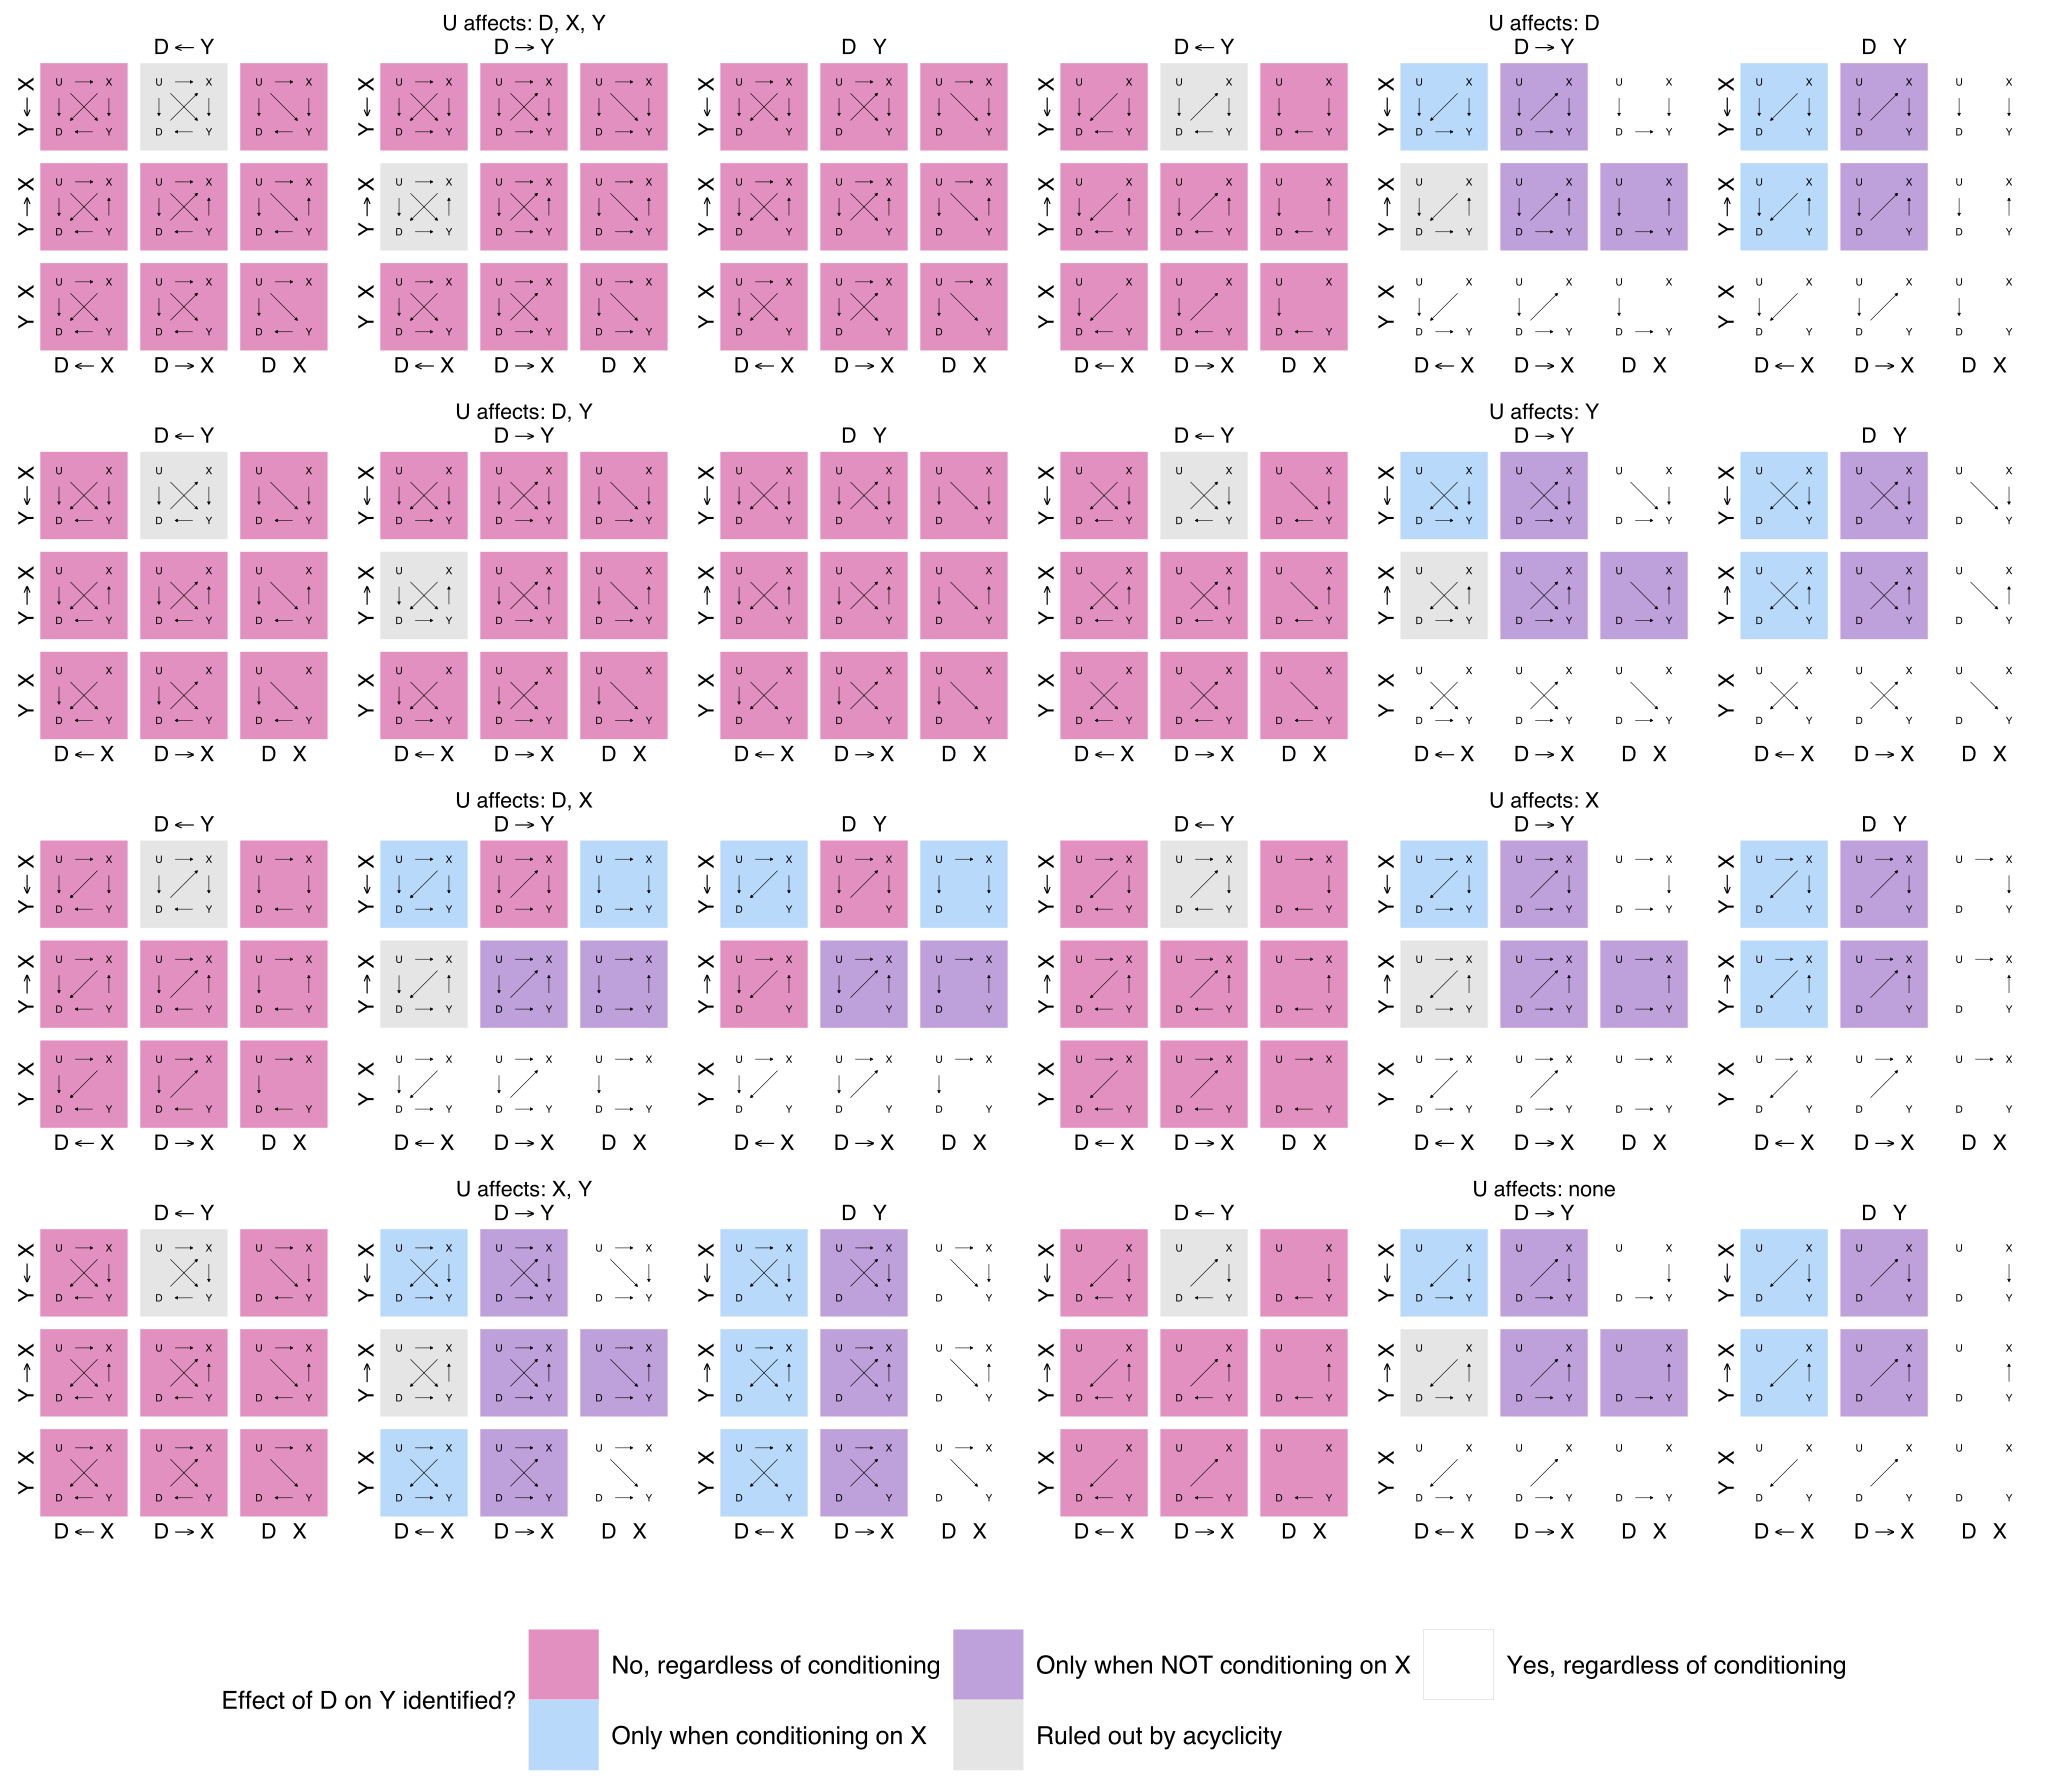
\includegraphics{05_Choosing_an_Answer_Strategy_files/figure-latex/dagsadjustment-1.pdf}
\caption{Consequences of conditioning on variable X for all 216 possible
DAGs.}
\end{figure}

\hypertarget{adding-model-based-assumptions}{%
\paragraph{Adding model-based
assumptions}\label{adding-model-based-assumptions}}

We can address the problem of unmeasured confounding by invoking
conditional independence assumptions. The ``selection-on-observables''
answer strategy invokes the assumption that \(D\) is statistically
independent of the potential outcomes of \(Y\) \emph{given} X,
i.e.~after adjusting for \(X\). In other words, controlling for \(X\)
blocks all backdoor paths between \(D\) and \(Y\). This assumption is
also known as a conditional independence or ignorability assumption.

In Figure @ref(fig:dagsignorability), we display the 216 possible causal
graphs again, ruling out in gray those that are cyclical. Among the 200
that remain, we color in the same way as under controlling for \(X\) but
add a fourth color: lavender for DAGs that we rule out based on our
conditional independence assumption. Those that are ruled out, in the
upper left quadrants, have unobserved confounding from \(U\) that cannot
be addressed by adjusting for \(X\).

Analysts who invoke this conditional independence assumption assure that
there are many fewer circumstances in which identification is not
possible either through controlling for \(X\) or not controlling for
\(X\). However, this is a strong assumption that is not possible to test
directly. Instead, the analyst must justify the assumption based on
circumstantial qualitative or quantitative evidence. The task is to rule
out through this evidence either a relationship between \(U\) and \(D\)
or a relationship between \(U\) and \(Y\) or both. In the first case,
this evidence might take the form of background knowledge about how
values of \(D\) are determined. The treatment might be assigned using a
cut-off rule, in which case all those above the cut-off are assigned to
treatment (e.g., are admitted to a college) and those below are not. In
this case, there is no relationship between unobserved variables \(U\)
and treatment \(D\), there is only a relationship between \(X\) (score)
and \(D\). Controlling for \(X\) will enable causal identification even
if \(Y\) is affected by \(U\). However, the assumption of conditional
independence between \(U\) and \(D\) given \(X\) is a strong assumption:
the analyst must be sure that there is no unobserved variable \(U\) that
directly affects \(D\), such as legacy applicants who may be ``pushed''
over the threshold of the cut-off if they are close enough to it.

Under selection-on-observables, there are still many DAGs that raise
problems for us. There are still many DAGs in which \(D\leftarrow Y\),
\(D\) is caused by \(Y\) instead of the other way around. If we cannot
rule those out by assumption, we will never identify the causal effect
of \(D\) on \(Y\) regardless of whether we control for \(X\). The DAGs
in blue (the effect is identified only when we condition on \(X\) and
not otherwise) and purple (the opposite, that we only achieve
identification when we do not condition on \(X\)) still remain. Those in
blue involve \(X\) confounding the relationship between \(D\) and \(Y\)
and those in purple are when \(X\) is a collider so conditioning on it
opens up a backdoor path to \(U\). In other words, the conditional
independence of \(D\) and \(U\) given \(X\) is insufficient to identify
the effect, without ruling out these other scenarios.

\begin{figure}
\centering
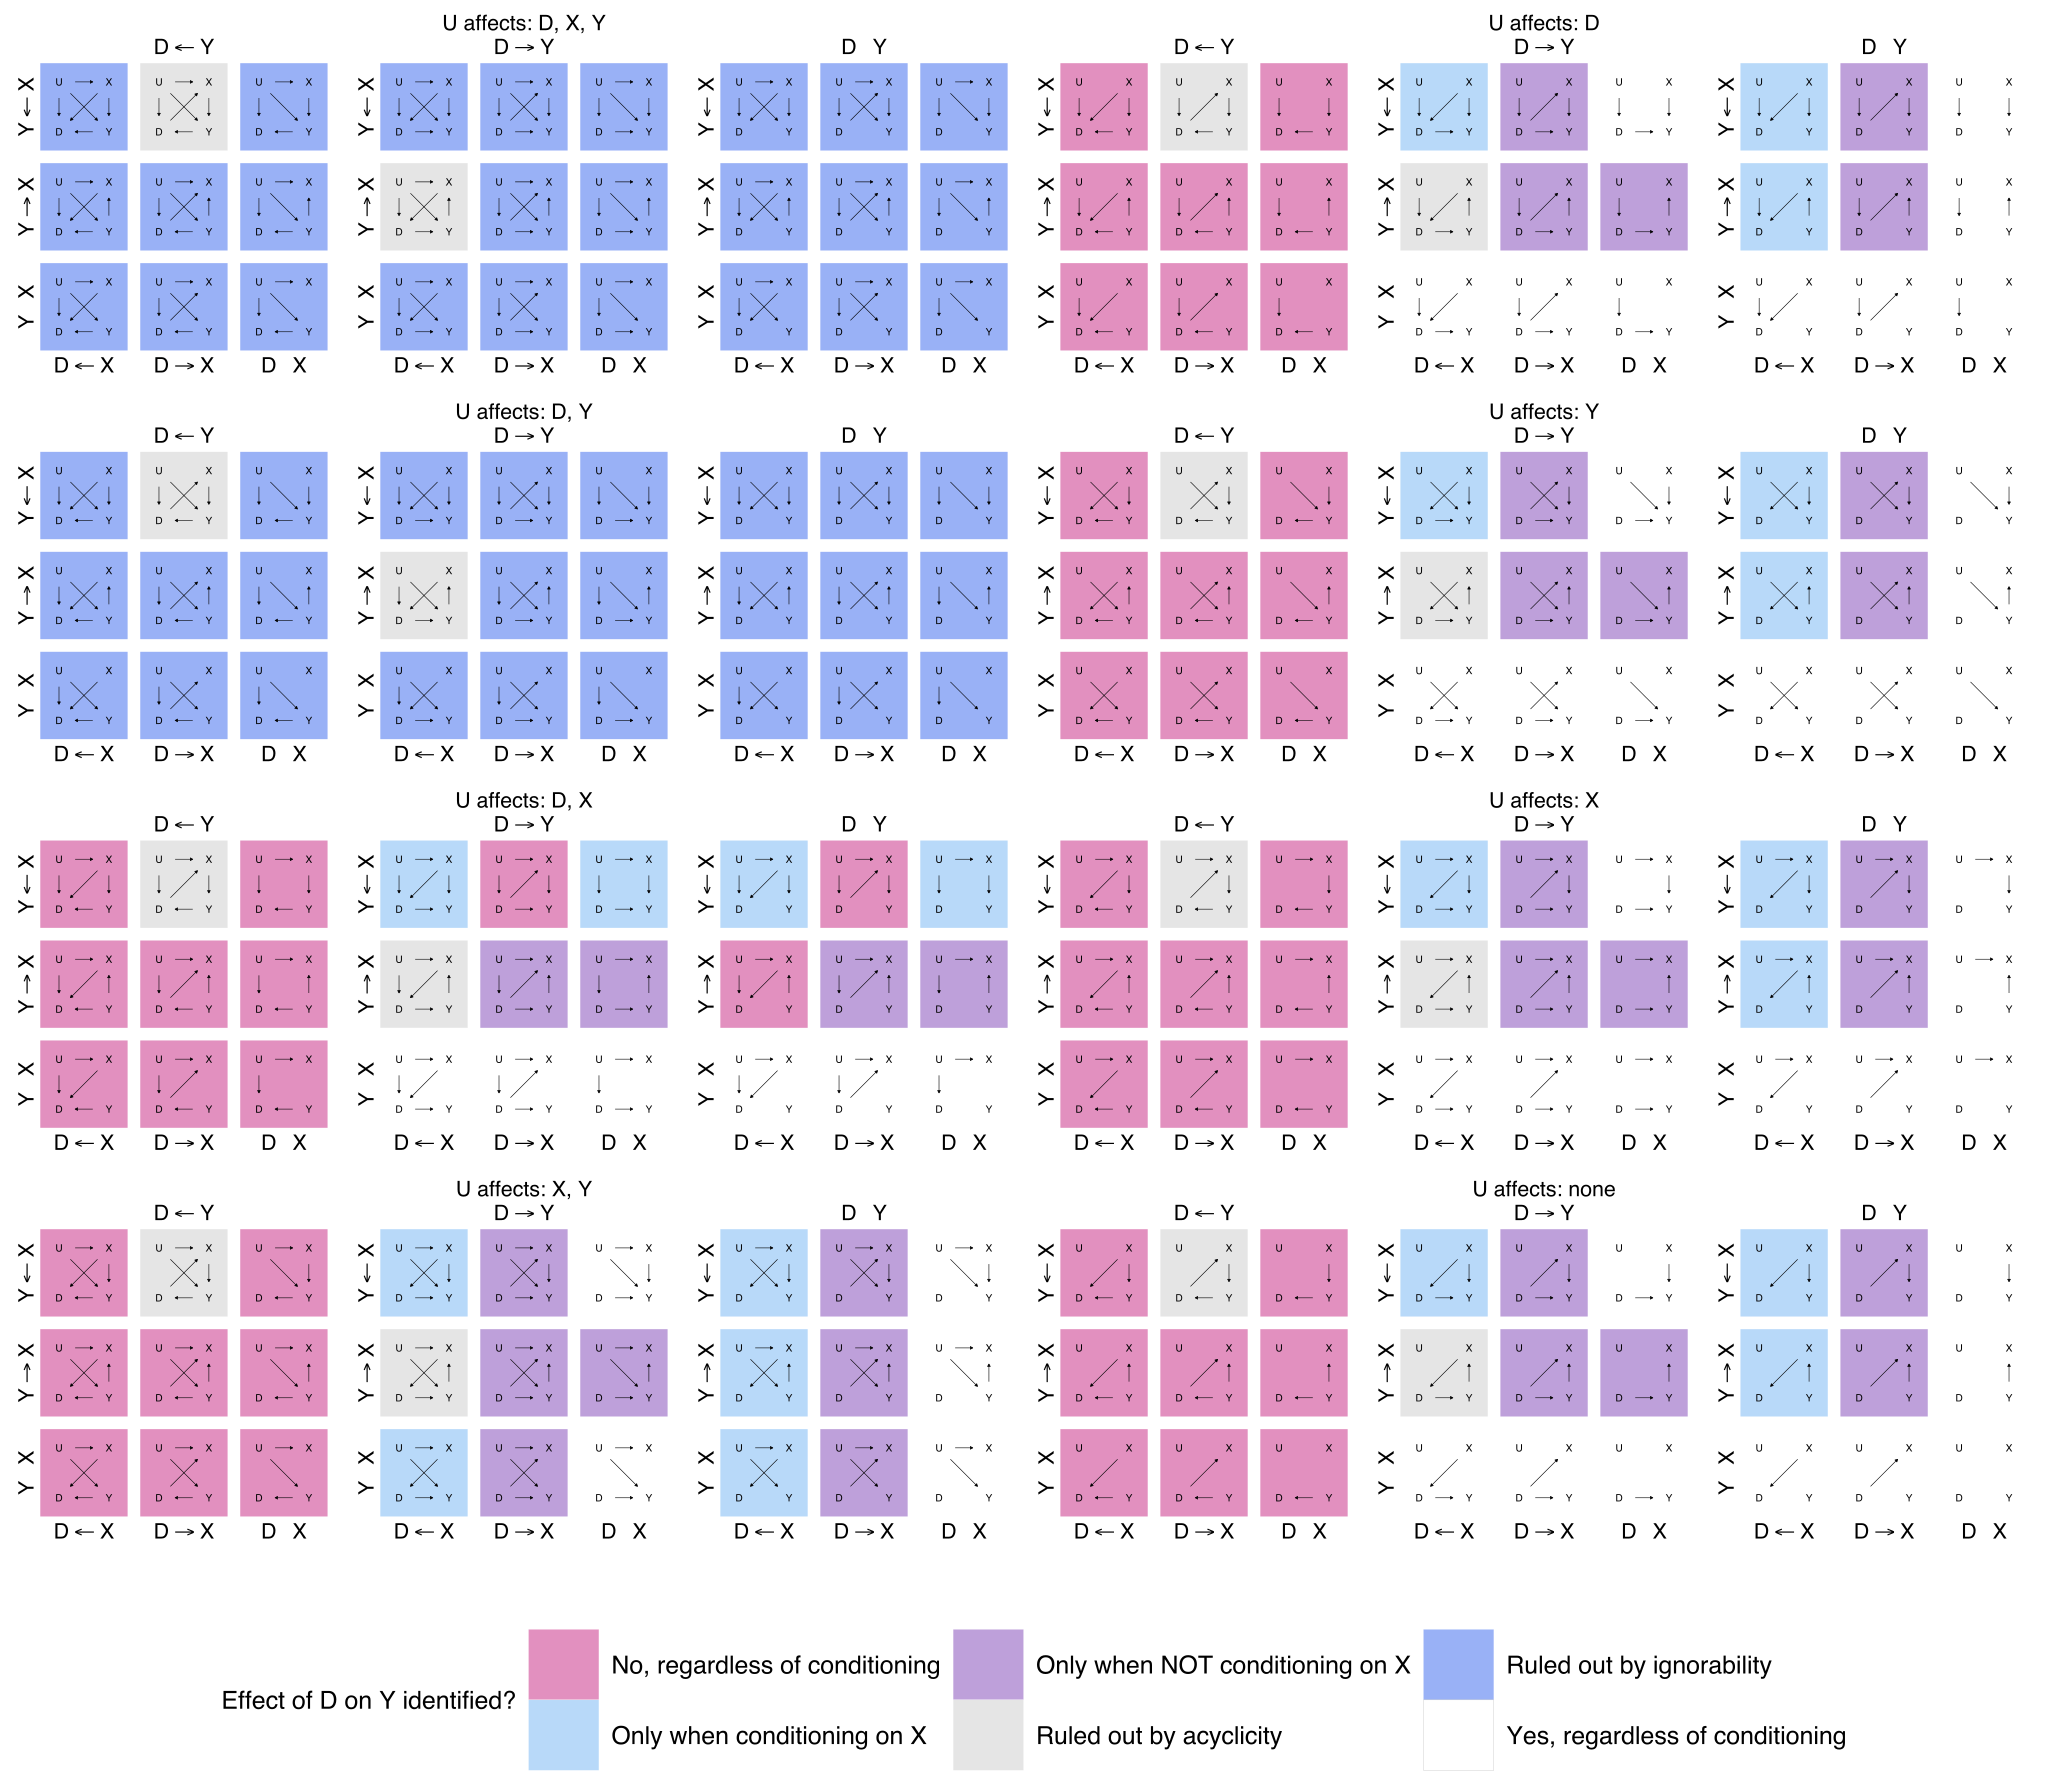
\includegraphics{05_Choosing_an_Answer_Strategy_files/figure-latex/dagsignorability-1.pdf}
\caption{Consequences of conditional ignorability assumption for all 216
possible DAGs.}
\end{figure}

\hypertarget{design-based-identification}{%
\paragraph{Design-based
identification}\label{design-based-identification}}

When we are unable to rule out confounding by assumption and adjustment,
we can randomly assign \(D\) to sever connections between unobserved
variables \(U\) and \(D\) by design. Ruling out confounders by
assumption or adjustment requires the \emph{model} to be correct, so is
often known as model-based inference, whereas ruling out confounders by
design is labeled design-based inference.\footnote{In truth, there is a
  continuum between the two. Design-based inferences that rely on
  non-parametric estimators of the average treatment effect using data
  from a randomized experiment are a classic design-based estimator, yet
  they also rely on a modeling assumption: the stable unit
  treatment-value assumption.} In addition, we can measure \(X\) before
treatment to rule out situations in which \(D\) causes \(X\), which can
lead to collider bias or opening backdoor paths from \(D\) to \(Y\).

In doing so, we dramatically reduce the set of possible DAGs, because we
set the causal order between \(X\) and \(D\), and dramatically expand
the number of settings under which the effect of \(D\) on \(Y\) is
identified both due to this restriction on causal order and the
randomization of \(D\) which guarantees ignorability of \(U\).

In Figure @ref(fig:dagsrandomization), we swap the colors to now
indicate DAGs ruled out by measuring \(X\) before treatment (salmon
squares), and those ruled out by random assignment (blue squares). In
all of the remaining white squares, the effect of \(D\) on \(Y\) is
causally identified, regardless of whether we adjust for \(X\) or not.
We remove the conditionality of inference depending on whether we
control. This is good, because ultimately even in the presence of strong
ignorability assumptions outlined in the last section there are many
possible DAGs in which controlling or failing to control lead to bias.
Now, our inferences do not depend on guessing the correct DAG.

\begin{figure}
\centering
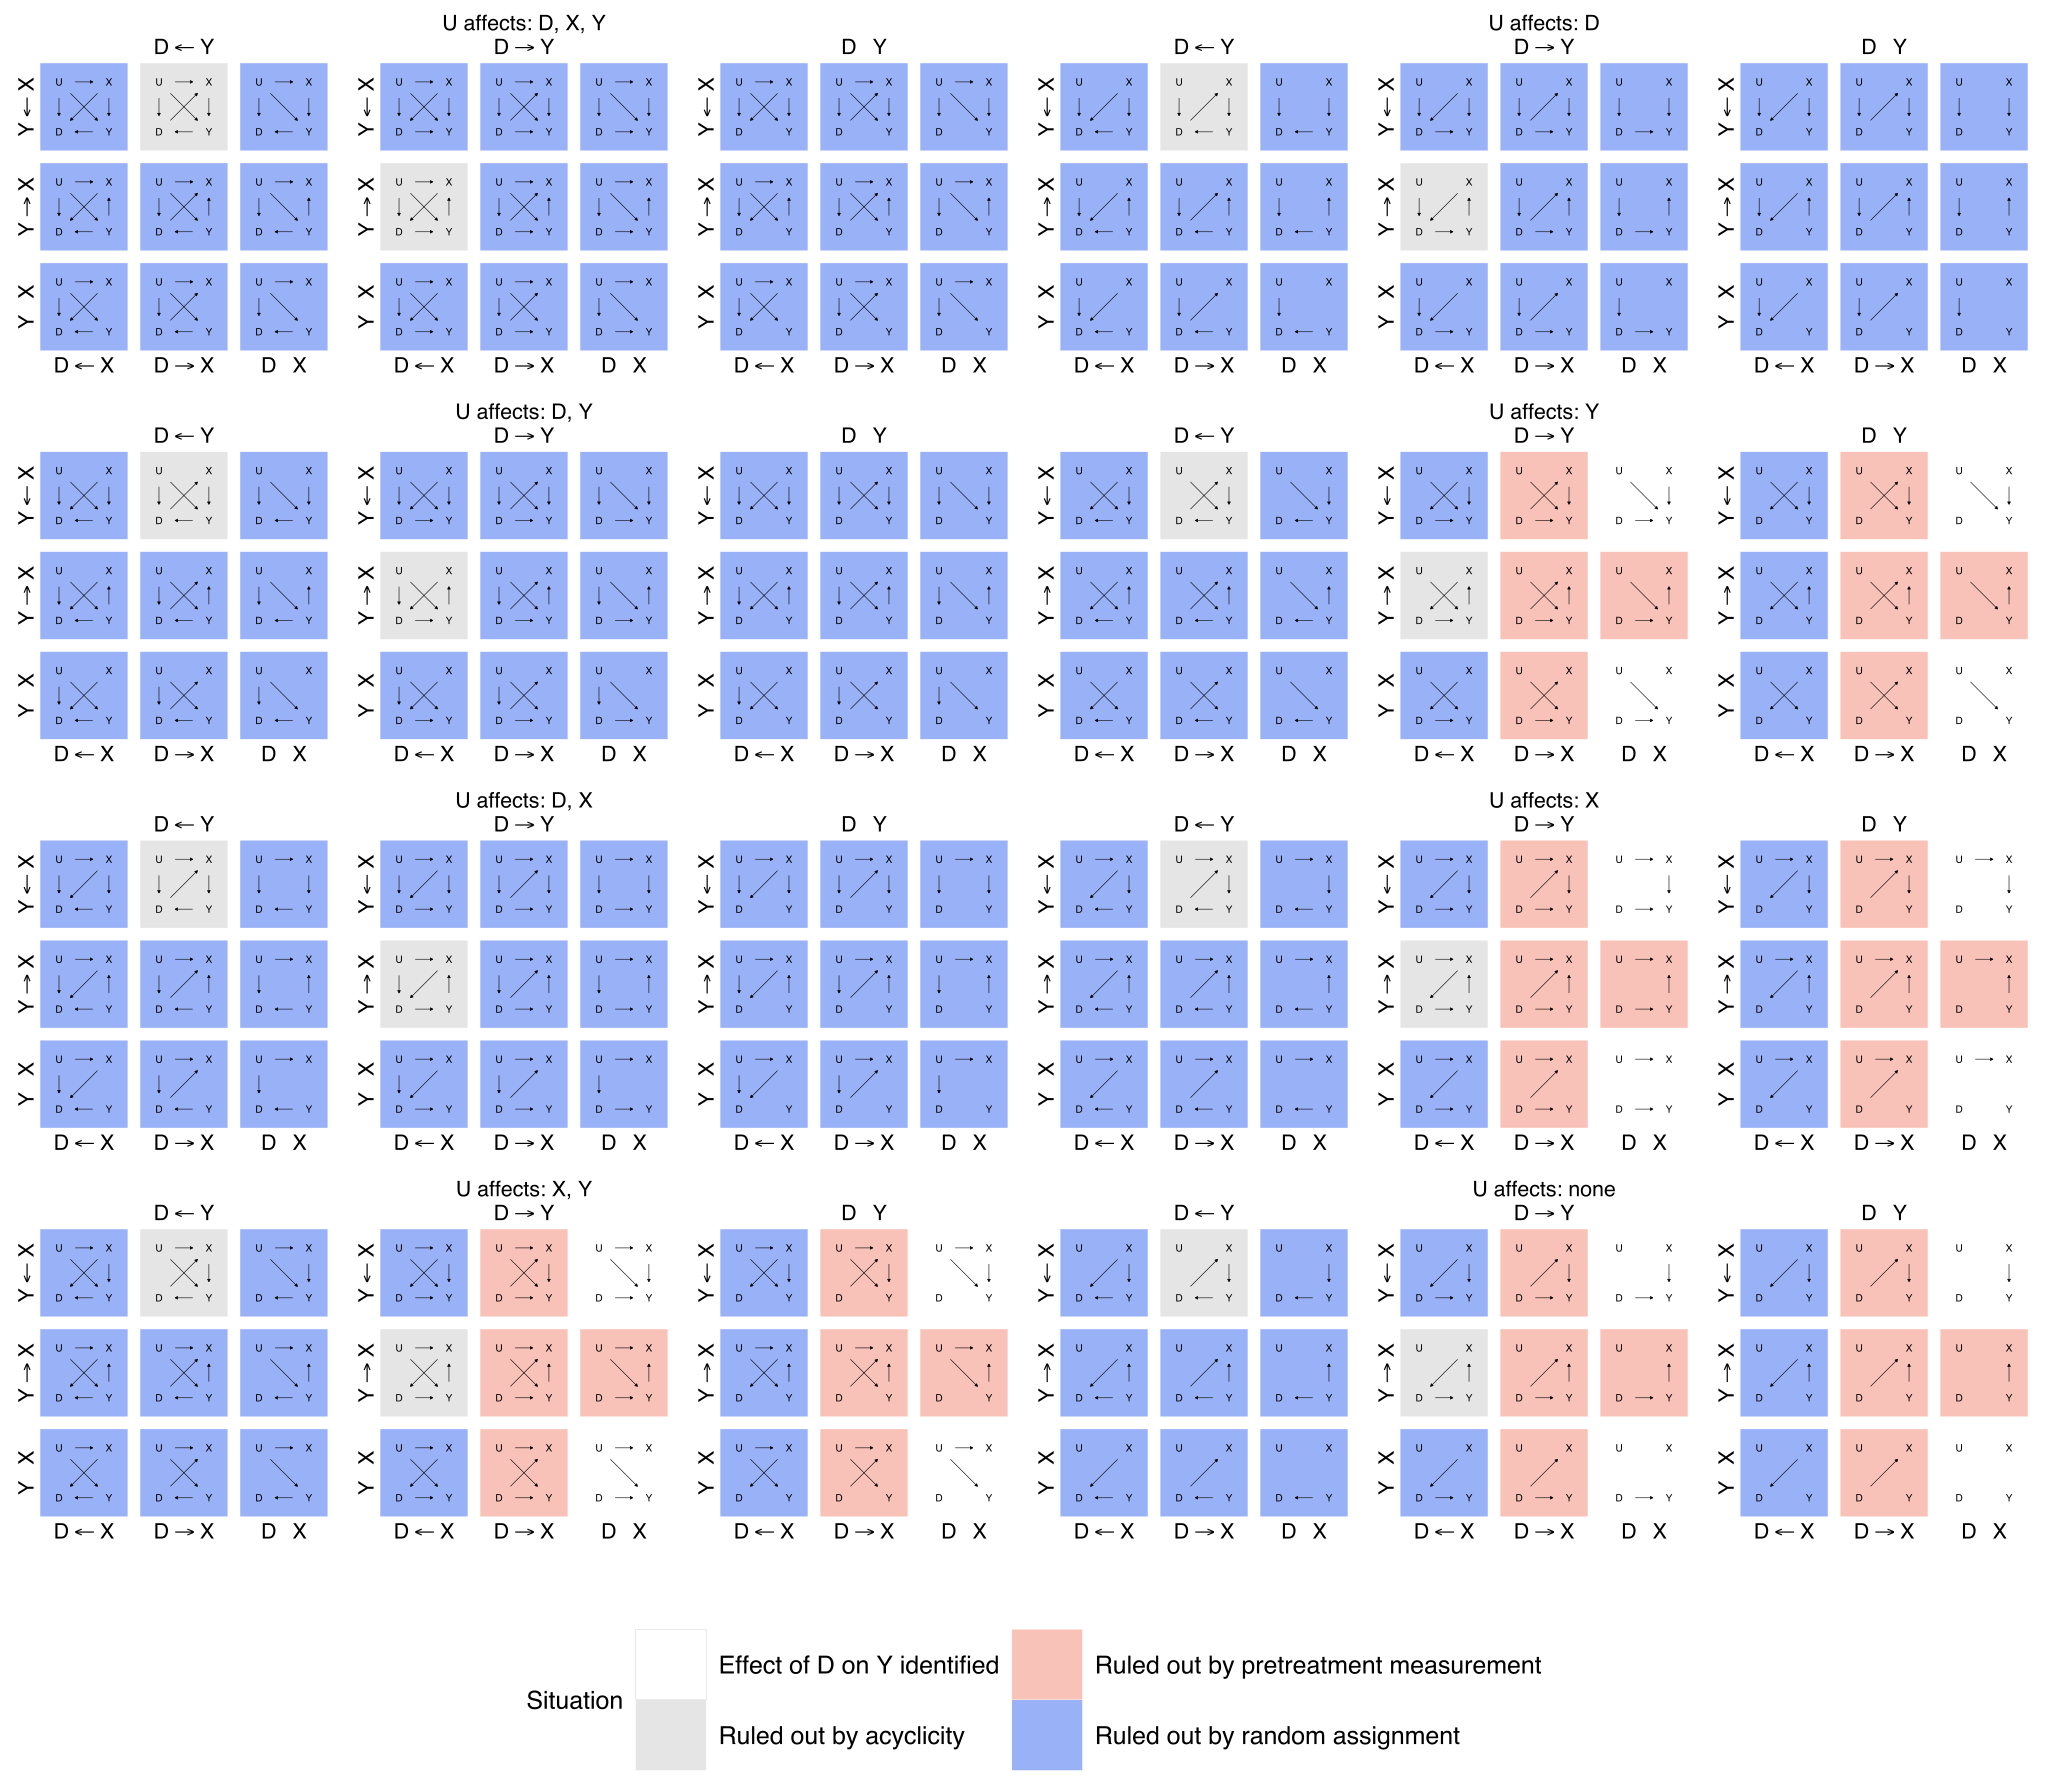
\includegraphics{05_Choosing_an_Answer_Strategy_files/figure-latex/dagsrandomization-1.pdf}
\caption{Consequences of randomizing Z and measuring X before treatment
for all 216 possible DAGs.}
\end{figure}

In short, what we do by controlling the timing of measurement of \(X\)
and randomizing \(D\) is to move our assumptions about conditional
independence from \(M\) our assumed (but possibly incorrect!) model of
the world into our data strategy, which we control and so can guarantee
by design.

\hypertarget{estimation}{%
\subsubsection{Estimation}\label{estimation}}

The identification of the causal effect of \(D\) on \(Y\) either by
assumption or design enables us to undertake two tasks: estimate the
average treatment effect, estimate the sign of the effect, or estimate
whether there is an affect or not.

The first task, estimating the magnitude of the effect of \(D\) on
\(Y\), can be accomplished using model-based inference under the
selection-on-observables design or under a randomized experiment. In
both cases, we apply the plug-in principle, replacing the true but
unknown average potential outcomes under treatment (control) with the
sample analogues, the average outcomes in the treatment (control) group.
With data from randomized experiments, \(X\) is ignorable, so we can
either adjust for it (which may reduce variability in estimates) or not
without bias. But under selection-on-observables, we have to rule out
many DAGs by assumption that include \(X\) as a collider or in which
\(X\) opens a backdoor path between \(D\) and \(Y\) in order to safely
select an answer strategy.

For estimating the sign of the effect, we can calculate the sign of the
effect magnitude, and then conduct a statistical test of the null
hypothesis of zero effect to distinguish among zero, positive, and
negative effects.

The third task, determining whether there is an effect or not, similarly
involves a statistical test of the null hypothesis of zero effect. If we
fail to reject the null, then our posterior belief is that there is no
effect, but if we reject in a two-sided test then we leave believing
there is an effect. This zero average effect null hypothesis test can
help us take the final step in distinguishing among the 216 possible
DAGs representing the relationships between \(D\) and \(Y\) and the
confounders \(X\) and \(U\). In Figure XX, we display the 16 DAGs that
are identified under random assignment and pretreatment measurement of
\(X\). We need to use data and the two-sided null hypothesis test to
distinguish between the top row (there is an effect \(D\rightarrow Y\))
and the bottom row (there is no effect). Our design got us most of the
way there, but then we need to use the data to narrow further to one of
the two rows of eight DAGs. Since our inquiry is about the causal
relationship between \(D\) and \(Y\), we may not be concerned about
distinguishing among the eight. If we are, we need to develop an
alternative research design in order to learn about the causal effects
of \(X\).

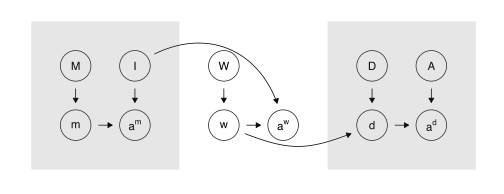
\includegraphics{05_Choosing_an_Answer_Strategy_files/figure-latex/unnamed-chunk-3-1.pdf}

\hypertarget{robustness}{%
\subsubsection{Robustness}\label{robustness}}

Robustness checks are modified answer strategies that aim to demonstrate
the ``robustness'' or ``sensitivity'' to answer strategy choices. Often
a primary analysis about a quantity of interest such as the effect of
treatment \(D\) on outcome \(Y\) is presented and then in an appendix a
set of modified analyses are presented. The author discusses whether or
not there is variation in the magnitude and statistical significance of
the estimates across these specifications.

Robustness checks are implicitly a response to the fundamental
uncertainty we identified in the last several sections over which is the
true DAG. We do not know! As a result, each robustness check should be
motivated by a particular DAG. When we complete a set of robustness
checks, we can then make claims about how ``robust'' our estimates of
the effect of \(D\) on \(Y\) are to alternative DAGs. Each robustness
analyses should aim to falsify a DAG, as in the case of controlling for
\(X\). If we have three variables \(X_1\), \(X_2\), and \(X_3\) that
either confound the relationship between \(D\) and \(Y\) or play no role
in the causal system, then we may want to present robustness checks
including and excluding each combination of the three variables. In
doing so, we rule out each variable as a collider or a mediator by
assumption. These analyses can help distinguish among DAGs and give us
evidence about the effect of \(D\) and \(Y\) across \emph{possible} DAGs
that involve confounding by some combination of \(X_1\), \(X_2\), and
\(X_3\). However, it is important to highlight the assumptions we make
in selecting the DAGs that are ruling in or out these relationships. In
order for controlling for \(X_2\) to be a sensible strategy, we must
invoke the assumption that \(X_2\) is not a collider. If it is possible
that it is, it is not clear what we can learn from adjusting for
\(X_2\). If we find its inclusion wipes out the effect of \(D\) on \(Y\)
this may not be because there is no causal relationship but because
\(X_2\) is a collider.

We illustrate with a simple analysis of the correlation between two
variables \texttt{y1} and \texttt{y2}, who have a true positive
correlation. \texttt{y2} is also a function of an observed covariate
\texttt{x} and measurement error. Our main analysis is a bivariate
regression predicting \texttt{y2} with \texttt{y1}. We compare this
answer strategy to one in which we run that analysis, but also run a
robustness check controlling for \texttt{x}. We do this because as the
analyst we are unsure of the true DGP and wish to demonstrate to
reviewer's that our results are not dependent on the functional form we
choose.

Using the MIDA way of thinking about designs, we discuss in the
diagnosis section another notion of the ``robustness'' of a design. The
typical way we think of robustness checks is multiple secondary analyses
\emph{conditional on the observed data} to build confidence in an
analysis of that fixed data. However, the motivation for these
robustness checks is uncertainty about the true data generating process.
By declaring a design in terms of MIDA, we can think about the
robustness of a \emph{single} estimator to multiple possible true data
generating processes. An estimator that is robust in this sense is one
that is unbiased with low uncertainty regardless of, say, the true
functional form between \texttt{y1} and \texttt{y2}. To determine
whether an estimator is robust, we can redefine a set of designs with
different functional forms and assess the rate of correct decisions of
our robustness checks strategy under each different model.

\hypertarget{following-the-inquiry}{%
\subsection{Following the inquiry}\label{following-the-inquiry}}

Answering descriptive inquiries involves studying the existence of nodes
and the values they take on. We might study whether a behavior exists in
the world, and measure its frequency. We might also study how the
frequency of the behavior varies over time and across people. Our answer
strategy, following the plug-in principle, will often involve the
average value of the node in the sample as an estimator of the average
value in the population.

By contrast, when we target a causal inquiry with our answer strategy,
we are interested in the existence (or non-existence) of an edge between
two nodes. We can label the two \(D\) (treatment) and \(Y\) (outcome).

\hypertarget{plug-in-principle}{%
\subsubsection{Plug-in principle}\label{plug-in-principle}}

The plug-in principle refers to the idea that good estiamtes of
population quantities \(I(m) = a^m\) can often be generated by choosing
an \(A\) that is very similar to \(I\) and then ``plugging-in'' \(d\)
for \(m\). Suppose that our inquiry is the average treatment effect
among the \(N\) units in the population.

\(I(m) = \frac{1}{N}\sum_1^N[Y_i(1) - Y_i(0)] = \frac{1}{N}\sum_1^NY_i(1) - \frac{1}{N}\sum_1^NY_i(0) = ATE\)

We can develop a plug-in estimator of the average treatment effect by
replacing the population means (\(\frac{1}{N}\sum_1^NY_i(1)\) and
\(\frac{1}{N}\sum_1^NY_i(0)\)) with sample analogues:

\(A(d) = \frac{1}{m}\sum_1^m{Y_i} - \frac{1}{N - m}\sum_{m+1}^N{Y_i}\),

where units 1 though \(m\) reveal their treated potential outcomes and
the remainder reveal their untreated potential outcomes. This
difference-in-means estimator of course depends on the strength of the
analogy between the population mean and the sample mean, which in turn
depends on features of the Data strategy. Under many (but not all) forms
of random assignment, the sample mean estimators of the treated and
untreated outcomes will be unbiased estimators. As discussed in Section
@ref(p2followdatastrategy), the specifics of the random assignment
strategy such as probabilities of assignment that vary by unit must be
taken into account.

More formally, Aronow and Miller describe a plug-in estimator as:

\begin{quote}
For i.i.d. random variables \(X_1, X_2, \ldots, X_n\) with common CDF
\(F\), the plug-in estimator of \(\theta = T(F)\) is:
\(\widehat\theta = T(\widehat F)\).
\end{quote}

\hypertarget{point-estimation}{%
\subsubsection{Point estimation}\label{point-estimation}}

Point estimation is possibly the most common class of answer strategy in
quantitative social science. Point estimators are things like the
difference-in-means, ordinary least squares regression, instrumental
variables regression, random forests, the LASSO, ridge regression,
BART\ldots{} the list goes on and on. These are the data analysis tools
taught in many graduate methods courses. What's incredible is that even
though the population of estimators proliferates with each passing year,
the number of kinds of inquiries they are useful for estimating stays
relatively flat. When we do point estimatation, we are mainly interested
in estimating averages, differences, variances, and conditional
expectation functions of increasing dimensionality. There are of course
many other kinds of estimands (like ratios and quantiles), but the main
point is, most of the variation in how scholars conduct point estimation
is in the answer strategy, not in the inquiry.

\begin{itemize}
\tightlist
\item
  Bias variance tradeoff
\item
  overfitting
\item
  add modeling assumptions that might decrease variance a lot at the
  cost of a little bias.
\item
  interacts with testing: could win on RMSE, but have a higher false
  positive rate.
\end{itemize}

(point people to Hastie and Tibshirani)

\hypertarget{estimating-the-variance}{%
\subsubsection{Estimating the variance}\label{estimating-the-variance}}

Variance estimation is often more difficult than point estimation.

We can often do the bootstrap, which plugs in (re-) sampling from the
sample for sampling from the population.

\hypertarget{tests}{%
\subsubsection{Tests}\label{tests}}

Tests are an elemental kind of answer strategy. Tests yield binary
yes/no answers to an inquiry. In some qualitative traditions, hoop
tests, straw-in-the-wind tests, smoking-gun tests, and doubly-decisive
tests are common. These tests are procedures for making analysis
decisions in a structured way. In frequentist statistics, significance
tests are used to make a decision whether to reject or fail to reject a
particular null hypothesis.

\hypertarget{partial-identification}{%
\subsubsection{Partial identification}\label{partial-identification}}

\begin{itemize}
\tightlist
\item
  confounding
\item
  EV bounds
\item
  trimming bounds
\end{itemize}

\hypertarget{p2followdatastrategy}{%
\subsection{Following the data strategy}\label{p2followdatastrategy}}

However, in order to benefit from these two controlled decisions in our
data strategy, we must follow the dictum due to R.A. Fisher to ``analyze
as you randomize.'' Your answer strategy should follow your data
strategy. There are four components: make comparisons only across
randomly-assigned conditions; analyze data at the level of random
assignment; make comparisons only in groups within which random
assignment was conducted (e.g., strata); and adjust for differences in
probabilities of random assignment. A parallel set of rules govern
answer strategies for descriptive inference: draw only on random samples
for describing a population; analyze data at the level of random
sampling (the primary sampling unit); and adjust for differences in
probabilities of sampling.

Making comparisons across randomly-assigned conditions within groups in
which random assignment was conducted directly follow from our
comparison of causal identification by assignment vs.~by design. If we
make comparisons that rely on differences both in \(D\) and \(X\), for
example a difference in treatment effects between two subgroups, we are
susceptible to confounding from \(U\), because \(X\) is not
randomly-assigned. Similarly, analysis of data from block-randomized
experiments can be broken by failing to account for blocking, because
blocks are not randomly assigned and in fact are typically constructed
so that the outcomes of units in the block are similar within blocks and
very different across blocks. If there are differential probabilities of
assignment across blocks and we pool our data ignoring the blocking
structure, our unweighted comparisons may be contrasting groups that
differ systematically. For descriptive inferences, we must always adjust
for different sampling inclusion probabilities.

In random sampling, the sampling probability quantifies each person's
likelihood of being in the sample. By taking the inverse of this
probability, we can generate weights that allow us to make a really
skewed sample representative of the target population. This basic
insight can be extended from random sampling to many other contexts. It
applies to random treatment assignment, where we use inverse probability
weighting to make unbiased inferences in the presence of spillovers and
heterogeneous assignment probabilities. It even extends to the use of
poststratification in nonrandom sampling and inverse propensity
weighting for unbiased causal inference in the presence of confounding.
For this reason, understanding the connection between sampling
probabilities and inverse probability weights is one of the most
important concepts in descriptive and causal inference. However, where
these weights come from and what they mean can often seem confusing. In
fact, the basic intuition is very simple and the random sampling analogy
extends directly to these other contexts.

When we sample, we select a subset of units to stand in for the
unselected units. That's what we mean when we say the sample is
``representative''---the units in it literally represent the units that
are not in it (but could have been). We can even quantify the exact
number of units in the population that each unit in the sample
represents. If I sample \(n = 10\) people from a group of \(N = 1000\)
people, then when I make an inference about the larger group from the
smaller group, each of the 10 people in the sample is standing in for
\(N/n = 100\) people in the population. If I sample all people, then
each person just represents one person, themselves: \(N/n = 1\). Let's
call \(w\) the number of people in the population each person in the
sample represents: \(w = N / n\). And let's call \(p\) the probability
of being in the sample: \(p = n / N\). Notice that \(p\) and \(w\) are
the reciprocal of one another. Since the number 1 divided by a fraction
gives its reciprocal, we can use the inverse of \(p\) to find \(w\):
\(\frac{1}{p} = \frac{1}{1} \times \frac{N}{n} = w\). Now you know what
an inverse probability weight is: it is a count of the number of people
in the population that a given unit in the sample represents.

Now suppose you have two samples, each of size \(n_1 = n_2 = 10\). The
first sample is drawn from a population of 10 people, each of whom has
\(X = 1\). The second sample is drawn from a population of 20 people,
each of whom has \(X = 0\). We want to know the true mean of \(X\)
across both populations:
\(\bar{X} = \frac{10 + 0}{10 + 20} = \frac{1}{3}\). If we pool the data
and take the average of \(X\), we get the wrong answer:
\(\hat{\bar{X}} = \frac{1}{2}\). We get the wrong answer because people
from the first group are overrepresented: while \(1/2\) of the sample is
from group 1, only \(1/3\) of the combined population is from group 1.
In terms of sampling probabilities and weights, every person in the
first sample only represents one person:
\(\frac{1}{p_1} = \frac{1}{1} \frac{N_1}{n_1} = \frac{1}{1} \frac{1}{1} = 1 = w_1\),
whereas every person in the second sample stands in for two people,
\(\frac{1}{p_2} = \frac{1}{1} \frac{20}{10} = 2 = w_2\). By weighting
our sample estimate of the average by the number of people each person
in the pooled sample represents, we recover the right answer:

\[\hat{\bar{X}}_{IPW} = \frac{\sum X_i w_i}{\sum w_i} = \frac{n_1 \times 1 \times w_1 + n_2 \times 0 \times w_2}{n_1 \times w_1 + n_2 \times w_2} = \frac{10 \times 1\times 1 + 10 \times 0 \times 2}{10 \times 1 + 10 \times 2} = \frac{1}{3} = \bar{X}.\]

Notice that this example is equivalent to a stratified random sampling
strategy, in which units from group 1 are sampled with \(p_1 = 1\) and
units from group 2 are sampled with probability \(p_2 = 1/2\). Any time
we use stratified random sampling and the probabilities vary among
strata, we should weight estimates so that each observation's
contribution is equivalent to the number of units it represents, which
corrects for any over- and underrepresentation introduced by the
sampling procedure.

This way of thinking provides a framework for poststratification on
nonrandom samples. Suppose a researcher comes across our dataset of 20
people. They don't know anything about the sampling strategy---to them,
it's a non-random sample. However, they do know that there are 10 people
from group 1 and 20 people from group 2 in the population, so they are
able to construct estimates of the sampling probabilities using
\(\hat{p_1} = n_1/N_1\) and \(\hat{p_2} = n_2/N_2\). From there, they
can construct weights using \(1/p_1\) and \(1/p_2\) that will reweight
their data so that it is representative. That's the basic intuition
behind \textit{post}stratification: you use known population counts to
reverse engineer the probability weights that a hypothetical stratified
random sampling strategy would have given you. See entry X in the design
library for more on this.

The analogy extends even further when we consider that all random
treatment assignment procedures are also sampling procedures. Rather
than sampling entire units, however, treatment assignments randomly
sample from different potential outcomes. If you assign 5/15 people to
treatment and the rest to control, for example, then the five treated
potential outcomes need to ``represent'' \(1/(5/15) = 3\) people's
treated potential outcomes and the ten people assigned to control
represent \(1/(10/15) = 1.5\) people's control potential outcomes. If
you tried to pool different experiments to get the average treatment
effect across all people in all experiments, you would need to take
account of the fact that different experiments might over or
underrepresent treatment or control potential outcomes, and weight
accordingly. This issue arises in block randomized designs where
treatment assignment probabilities vary by block (see entry X in the
design library), in designs with spillovers where spatial networks
induce differential assignment probabilities for spillovers (see entry X
in the design library), and in stepped wedge designs where earlier waves
overrepresent control potential outcomes and later waves overrepresent
treatment potential outcomes (see entry X in the design library).
Finally, in the same way that poststratification uses covariates to
construct sample weights corresponding to a hypothetical random
\textit{sampling} procedure, matching and selection observable designs
use covariates to reverse engineer probabilities of sampling treatment
and control potential outcomes in order to reweight the data to account
for the systematic selection of certain kinds of units into or out of
treatment (confounding).

\hypertarget{qualitative-methods-of-inference}{%
\subsection{Qualitative methods of
inference}\label{qualitative-methods-of-inference}}

When seeking to answer causal attribution inquiries about whether a
postulated cause was really necessary or sufficient to produce an
outcome (Section @ref(causalattribution)), most scholars turn toward
qualitative answer strategies {[}mahoneygoertz2004{]}. So it is no
surprise that many qualitative methods focus on tools to explore
necessity and sufficiency through probabilistic and deterministic logic.
However, it is important to distinguish between answer strategies and
inquiries. Just as there are quantitative strategies that target causal
attribution inquiries (Yamamoto 2012), there are qualitative answer
strategies that can be used to understand inquiries about causal
effects.

\hypertarget{process-tracing}{%
\subsubsection{Process-tracing}\label{process-tracing}}

Process-tracing is a term that has been used to describe approaches to
descriptive inference and theory-building exercises (Beach and Pedersen
2013, 13), but it is increasingly prominent as an approach to causal
inference (Collier 2011, 824).

\hypertarget{boolean-and-set-theoretic-methods}{%
\subsubsection{Boolean and set-theoretic
methods}\label{boolean-and-set-theoretic-methods}}

\hypertarget{narrative-comparison}{%
\subsubsection{Narrative comparison}\label{narrative-comparison}}

\hypertarget{answer-strategies-as-procedures}{%
\subsection{Answer strategies as
procedures}\label{answer-strategies-as-procedures}}

Consider a randomized experiment that seeks to estimate the causal
effect of a treatment. The answer strategy is not just ``Logistic
Regression with Covariate adjustment''. It includes every step in the
process that takes the raw data, cleans and recodes it, considers 5
alternative estimators (DIM, OLS with covariate adjustment, a fancy
thing your colleague suggested but you couldn't get to converge), before
finally settling on logit.

\textbf{Multiple estimates.} Answer strategies can account how many
statistical tests you are conducting. Often, when generating an answer
to a single inquiry, we may construct multiple estimates that provide
different types of answers of varying quality. When you present the
results from many null hypothesis tests, the rate of falsely rejecting
at least one of those tests even when all are true goes up, due to the
multiple comparisons problem. If you plan to adjust for this problem,
those adjustments are part of your answer strategy, because they will
typically adjust the p-values you report and the decisions readers make
with them. We may have three survey items that imperfectly estimate a
latent quantity. In presenting the results, we could present three
estimates from three regressions, we could adjust the three estimates
using a procedure such as a family-wise error rate correction, or we
could average the three items together into an index and present one
estimate from one regression. Which of these three methods we select
will change the properties of our answer strategy.

\textbf{Analysis procedures}. The final estimator that goes into a paper
is neither the beginning nor the end of the answer strategy. Procedures,
if any, by which you explore the data and determine a final set of
estimates are part of the answer strategy. Procedures for summarizing
multiple estimates are one example of many.

Commonly, the final estimator that is selected depended on a exploratory
procedure in which multiple models are assessed, for example by
comparing model fit statistics. The answer strategy of our research
design is not to fit the final model --- is it this multiple step
if-then procedure. These procedures may be part of a prespecified
analysis plan or they may be informal, so it may sometimes only be
possible to declare the full design after the data is obtained. (We may
find that a different analysis procedure that was not data dependent
would have been preferable, if we diagnose the design after the fact.)
The reason to declare the procedure rather than the final estimator is
that the diagnosis of the design may differ. The procedure may be more
powerful, if for example we assessed multiple sets of covariate controls
and selecting the specification with the lowest standard error of the
estimate. But the procedure may also exhibit poor coverage, accounting
for these multiple bites at the apple.

We also sometimes find that the model we planned to run to analyze the
data cannot be estimated. In these cases, there is an iterative
estimation procedure in which a first model is run, changes to the
specification are made, and a second or third model is presented as the
result. The full set of steps --- a decision tree, depending on what is
estimable --- is the answer strategy and we can evaluate whether it is a
good one not only under the realized data but under other possible
realizations where the decision \emph{tree} would be the same but the
decisions different.

In fact, there are examples of analysis procedures in most types of
research, quantitative or qualitative. Many strategies for causal
inference with observational data involve not only an estimation
strategy but a set of falsification or placebo tests. The answer
provided by these research designs depends in a crucial way on the
results of these tests: if the tests fail, the design provides no
definitive answer. In qualitative research, process tracing involves a
set of steps, the results of which depend on information gathered in
earlier steps. Many mixed methods strategies are also multi-step
procedures. Nested designs involve running a quantitative analysis and
then selecting cases on the basis of predictions from the regression.
These designs cannot be assessed by considering a single step of the
procedure in isolation.

\textbf{When things do not go according to plan.} To compare answer
strategies, you can imagine the estimators that are possible \emph{if
things go well} as well as \emph{if things go wrong}, when there is
missing data or there are outliers in variables. A good answer strategy,
which might be a single estimator, or a procedure if-this-then-that, can
handle both states of the world. Procedures for addressing deviations
from expected analyses are part of the answer strategy. Even in the
absence of a preanalysis plan, we often have a way we expect to analyze
the data if things go well. When they do not --- because data are
missing, there is noncompliance with an intervention, or the study is
suspended for example --- the answers will change. These procedures
determine the answer the study provides (or in some cases does not), so
are part of the answer strategy. \emph{Standard operating procedures}
(lin and green) are documents that systematize these procedures in
advance.

We demonstrate the fact that the properties of procedures differ from
the properties of a design with the final estimator in a simple example.
We compare two possible estimation specifications, with and without
covariates, to a procedure in which we run both models and report the
model in our paper that has the lower p-value. The models are exactly
the same, but the properties of the \emph{procedure} differ from the
properties of either of the two possible models. In particular, the
procedure has higher power than either of the two models, but it
exhibits poor coverage, which means we have a bias in our measure of
uncertainty.

\hypertarget{interpretation}{%
\subsection{Interpretation}\label{interpretation}}

The answer strategies we have described thus far also yield a single
answer, whether it is a point estimate, a set of bounds, or a p-value.
Yet these take up only a tiny proportion of the writeup of a study's
results. Much more ink is taken up by the tables that report on them,
the figures that visualize them, and the results and discussion sections
that describe them. Importantly, how we report, visualize, and describe
results will change depending on the realization of the data. These
choices often depend on the results both in simple ways, such as the
scale of the outcomes changing, and in more complex ways, such as
whether a result is even reported on in the paper if it is not
statistically significant.

How we report, visualize, and describe results is part of the answer
strategy. What answer we provide to readers depends on these components,
and not only the numbers that pop out of our regression. Considering how
these aspects of our answer strategy change depending on how the data
strategy turns out

\hypertarget{further-reading}{%
\subsection{Further reading}\label{further-reading}}

\begin{itemize}
\tightlist
\item
  Gelman and Hill (2006) and {[}other stories{]} on multilevel modeling.
\item
  Aronow and Samii (2016) on the generalizability of regression
  estimators in observational settings.
\item
  Van Evera (1997) on hoop tests.
\end{itemize}

\hypertarget{refs}{}
\leavevmode\hypertarget{ref-aronow2016does}{}%
Aronow, Peter M., and Cyrus Samii. 2016. ``Does Regression Produce
Representative Estimates of Causal Effects?'' \emph{American Journal of
Political Science} 60 (1): 250--67.

\leavevmode\hypertarget{ref-beachpedersen2013process}{}%
Beach, Derek, and Rasmus Brun Pedersen. 2013. \emph{Process-Tracing
Methods: Foundations and Guidelines}. University of Michigan Press.

\leavevmode\hypertarget{ref-collier2011understanding}{}%
Collier, David. 2011. ``Understanding Process Tracing.'' \emph{PS:
Political Science \& Politics} 44 (4): 823--30.

\leavevmode\hypertarget{ref-gelman2006data}{}%
Gelman, Andrew, and Jennifer Hill. 2006. \emph{Data Analysis Using
Regression and Multilevel/Hierarchical Models}. Cambridge: Cambridge
University Press.

\leavevmode\hypertarget{ref-VanEvera1997}{}%
Van Evera, Stephen. 1997. \emph{Guide to Methods for Students of
Political Science}. Ithaca: Cornell University Press.

\leavevmode\hypertarget{ref-yamamoto2012understanding}{}%
Yamamoto, Teppei. 2012. ``Understanding the Past: Statistical Analysis
of Causal Attribution.'' \emph{American Journal of Political Science} 56
(1): 237--56.

\end{document}
